
\documentclass[a4paper,12pt]{scrbook}
\usepackage{amsmath,amssymb,amsthm}
\usepackage{fancyvrb}
\usepackage{parskip}
\usepackage{lastpage}
\usepackage{verbatim,boxedminipage,enumitem}
\usepackage{ifthen}
\usepackage{color,graphicx}
\usepackage{pgf}
\usepackage{longtable}
\usepackage{upquote}
%\usepackage[all]{xy}
\usepackage{tobiShell}
\usepackage{tikz}
\usetikzlibrary{automata}
\usetikzlibrary{arrows}
\usepackage{pgf,pgfarrows,pgfnodes}
\usepackage{pgfplots}
\usepackage{circuitikz}
\usetikzlibrary{circuits}
\usetikzlibrary{circuits.logic.US}
\usepackage{mymath}
\usepackage{python}
%------------------------------------------------------------------
% Verbatim for console window - single line frame, no line numbers
%------------------------------------------------------------------
\DefineVerbatimEnvironment%
 {console}{Verbatim}
 {frame=single}

%--------------------------------------------------------
% Remove the vertical spacing before and after Verbatim.
%--------------------------------------------------------
\usepackage{atbeginend}
\BeforeBegin{console}{\mbox{}\\ \begin{minipage}{\textwidth}\vspace{3pt}}
\AfterEnd{console}{\vspace{4pt} \end{minipage} \\ }

\begin{document}
\thispagestyle{empty}

\begin{center}
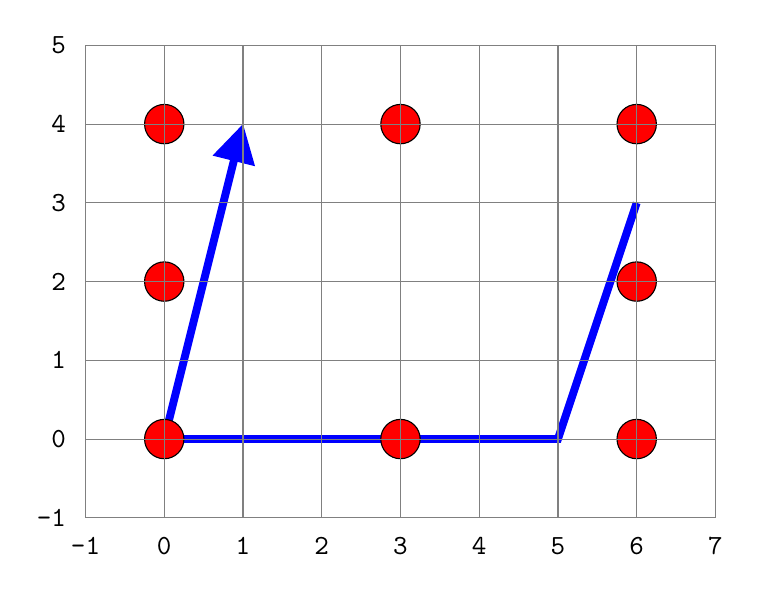
\begin{tikzpicture}
\draw[line width=0.1cm,blue,<-,>=triangle 60] (1,4) -- (0,0) -- (5,0) -- (6,3);
\fill[blue] (6, 3) circle (0);

\draw[blue] (6, 3)
circle (0.0);
\fill[red] (3.0, 4.0) circle (0.25);

\draw[black] (3.0, 4.0)
circle (0.25);
\fill[red] (3.0, 0.0) circle (0.25);

\draw[black] (3.0, 0.0)
circle (0.25);
\fill[red] (0.0, 2.0) circle (0.25);

\draw[black] (0.0, 2.0)
circle (0.25);
\fill[red] (6.0, 2.0) circle (0.25);

\draw[black] (6.0, 2.0)
circle (0.25);
\fill[red] (0.0, 4.0) circle (0.25);

\draw[black] (0.0, 4.0)
circle (0.25);
\fill[red] (6.0, 4.0) circle (0.25);

\draw[black] (6.0, 4.0)
circle (0.25);
\fill[red] (0.0, 0.0) circle (0.25);

\draw[black] (0.0, 0.0)
circle (0.25);
\fill[red] (6.0, 0.0) circle (0.25);

\draw[black] (6.0, 0.0)
circle (0.25);
\draw[gray] (-1.0,-1.0) -- (-1.0,5);
\draw[gray] (0.0,-1.0) -- (0.0,5);
\draw[gray] (1.0,-1.0) -- (1.0,5);
\draw[gray] (2.0,-1.0) -- (2.0,5);
\draw[gray] (3.0,-1.0) -- (3.0,5);
\draw[gray] (4.0,-1.0) -- (4.0,5);
\draw[gray] (5.0,-1.0) -- (5.0,5);
\draw[gray] (6.0,-1.0) -- (6.0,5);
\draw[gray] (7.0,-1.0) -- (7.0,5);
\draw[gray] (-1.0,-1.0) -- (7,-1.0);
\draw[gray] (-1.0,0.0) -- (7,0.0);
\draw[gray] (-1.0,1.0) -- (7,1.0);
\draw[gray] (-1.0,2.0) -- (7,2.0);
\draw[gray] (-1.0,3.0) -- (7,3.0);
\draw[gray] (-1.0,4.0) -- (7,4.0);
\draw[gray] (-1.0,5.0) -- (7,5.0);
\draw(-1, -1) node [font=\ttfamily, label=below:{\texttt{-1}}] {};
\draw(0, -1) node [font=\ttfamily, label=below:{\texttt{0}}] {};
\draw(1, -1) node [font=\ttfamily, label=below:{\texttt{1}}] {};
\draw(2, -1) node [font=\ttfamily, label=below:{\texttt{2}}] {};
\draw(3, -1) node [font=\ttfamily, label=below:{\texttt{3}}] {};
\draw(4, -1) node [font=\ttfamily, label=below:{\texttt{4}}] {};
\draw(5, -1) node [font=\ttfamily, label=below:{\texttt{5}}] {};
\draw(6, -1) node [font=\ttfamily, label=below:{\texttt{6}}] {};
\draw(7, -1) node [font=\ttfamily, label=below:{\texttt{7}}] {};
\draw(-1, -1) node [font=\ttfamily, label=left:{\texttt{-1}}] {};
\draw(-1, 0) node [font=\ttfamily, label=left:{\texttt{0}}] {};
\draw(-1, 1) node [font=\ttfamily, label=left:{\texttt{1}}] {};
\draw(-1, 2) node [font=\ttfamily, label=left:{\texttt{2}}] {};
\draw(-1, 3) node [font=\ttfamily, label=left:{\texttt{3}}] {};
\draw(-1, 4) node [font=\ttfamily, label=left:{\texttt{4}}] {};
\draw(-1, 5) node [font=\ttfamily, label=left:{\texttt{5}}] {};
\end{tikzpicture}

\end{center}

\end{document}
